\section{Latency in Cellular Networks}

\subsection{Methodology and Experiment}
\label{sec:methodology}

There are several existing tools for measuring mobile network performance \cite{speedtest, huang2011mobiperf}; however, these techniques are often too narrow in scope and can only be applied in a limited manner. We shy away from developing a whole new suite of measurement tools for mobile contexts given the fact that there are many general tools for understanding network performance (\ref{sec:tools}). We aim to reuse these existing tools in our study. We utilize mobile devices (in this case a smart phone) as a tethered network interface to a measurement system. The mobile device will serve as the first hop, allowing use to use existing tools and techniques to perform measurements. We utilize USB tethering to minimize the possibility of interference. As we will show in our data analysis, the latency of the first hop is negligible. Fig.\,\ref{fig:mobile_networks_method} illustrates our technique for probing cellular networks.

\begin{figure}
  \centering
  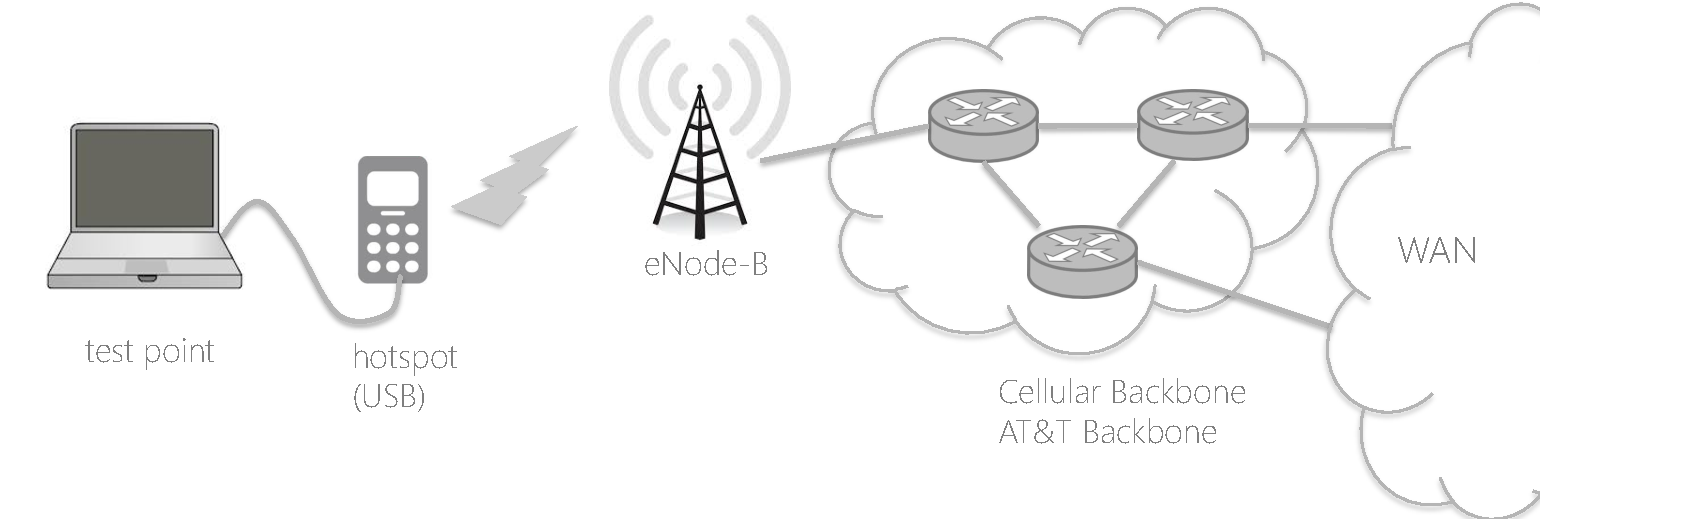
\includegraphics[width=\linewidth]{../figs/mobile_networks_method.pdf}
  \vspace{-1em}
  \caption{Mobile device USB tethered computer to perform {\textit traceroute}. This allows us to calculate the per-hop latency in cellular backbone.}
  \label{fig:mobile_networks_method}
\end{figure}

We utilize {\textit traceroute} to quantify the latency for each hop within cellular networks. The targets for {\textit traceroute} are the top 1000 websites. Since we are only interested in the cellular backbone networks, we limit the maximum hop count of {\textit traceroute} to 13. We also perform Autonomous System Number (ASN) lookups for each hop encountered. Fig.\,\ref{fig:traceroute} shows an example trace to Google.

\begin{figure}[!htb]
  \centering
  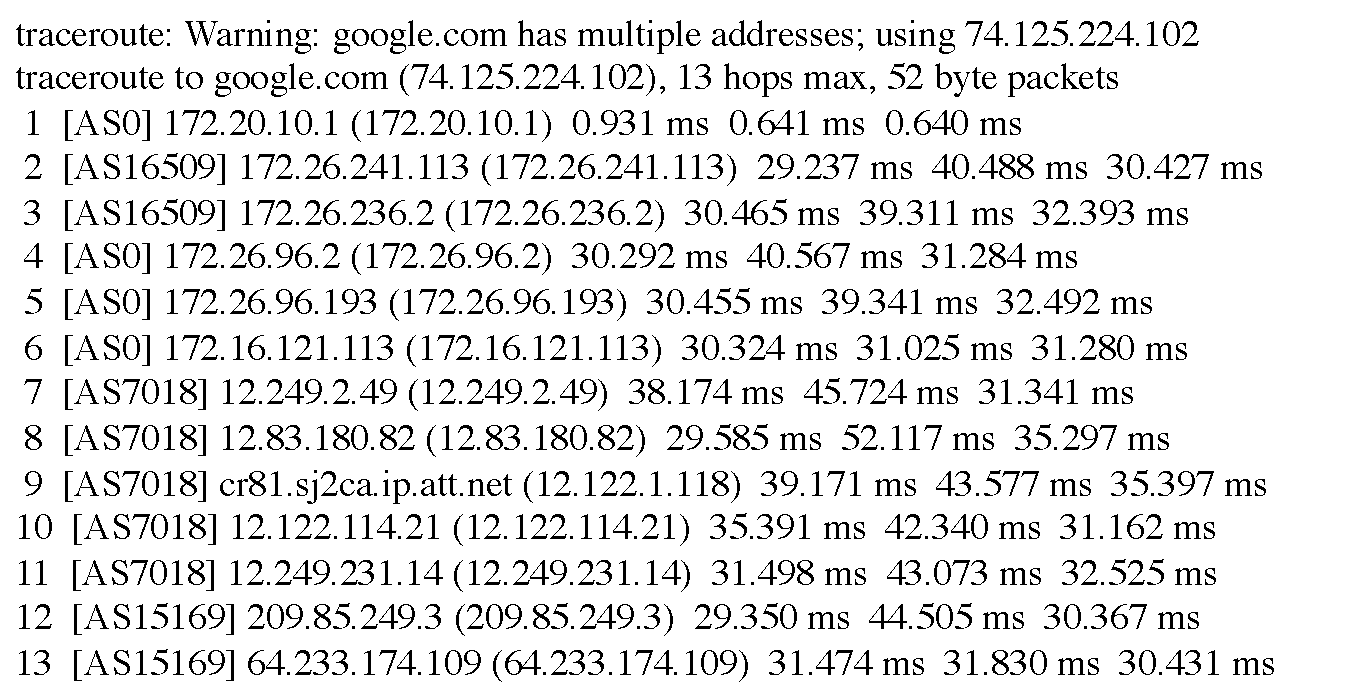
\includegraphics[width=1.1\linewidth]{../figs/traceroute.pdf}
  \vspace{-1em}
  \caption{Example {\textit traceroute} log from an AT\&T iPhone in Berkeley, maximum hop limited to 13, with ASN look-up turned on.}
  \label{fig:traceroute}
\end{figure}


The measurement was conducted between Apr.\,11 and Apr.\,24 (during periods in which we had access to a modem device). In total we have collected 191886 measurements, with each including a timestamp, received signal strength indication (RSSI), radio type (LTE or 4G-LTE), the traceroute hop number, ASN, hostname, host IP, and the specific delay. It is worth mentioning that the timestamp, RSSI and radio type are the same for each measurement. The reason is due to the difficulty in accessing RSSI and radio type programmatically. The we must manually record this data when performing the measurements.

Over the course of the experiment, we performed measurements while driving to and from San Francisco (SF). We expand on these results in the analysis section. 

\subsection{Analysis}
\label{sec:analysis}

We being with an example trace to Google (Fig.\,\ref{fig:traceroute}). As you can see, the first hop has an IP address $172.20.10.1$, and latencies 0.931 ms, 0.641 ms, 0.640 ms; this is the iPhone used for USB hotspot. Throughout the experiment, the latency introduced by this USB link is generally small, within 1 ms. Then the second hop reaches out to the first layer 3 router within AT\&T's cellular network. In the LTE architecture, the Evolved Node B (eNode-B) (Fig.\,\ref{fig:mobile_networks_method}) communicates directly with User Equipment (UEs), but it does not have layer 3 semantics. It is the access gateway (AGW) \footnote{AGW also provides termination of the LTE bearer, acts as a mobility anchor point for the user plane. Other key logical functions including MME (Mobility Management Entity) for the Control Plane and SAE PDN GW (System Architecture Evolution Packet Data Network GateWay) for the User Plane \cite{nortel}} that works on IP layer. Afterwards, the packet will enter AT\&T's cellular backbone, traversing routers either with private IP -- 172.16/12 \cite{rekhterrfc}, or with AT\&T's prefix -- 12/8. Interestingly, the ASN reported by {\textit traceroute} on the second and third hop is from Amazon's AS (AS16509). This might be due to some incorrect information in the ASN look-up. At hop 12, the route exits AT\&T's network and enters Google's AS.

This same pattern holds for many other traces. We aggregate them to answer the following question: what are the properties of AT\&T's cellular backbone? Is the latency stable, and are the routes stable? We plot the graph in Fig\,\ref{fig:mobile_latency}. The top figure shows the latency experienced on each hop (the horizontal axis is hop number, and vertical axis is latency in milliseconds). The red bar is the mean value for each hop, and the blue error bar is 5th and 95th percentile. We have also noted the mean value on top of each bar. The bottom figure displays the routing stability within the cellular networks. We mark each different router IP in a unique color for each hop. the portion of that color within each bar represents the portion of {\textit traceroute} responses received from that router for that hop. Again, it is important to note that the first hop is the iPhone through USB tethering.

\begin{figure}
  \centering
  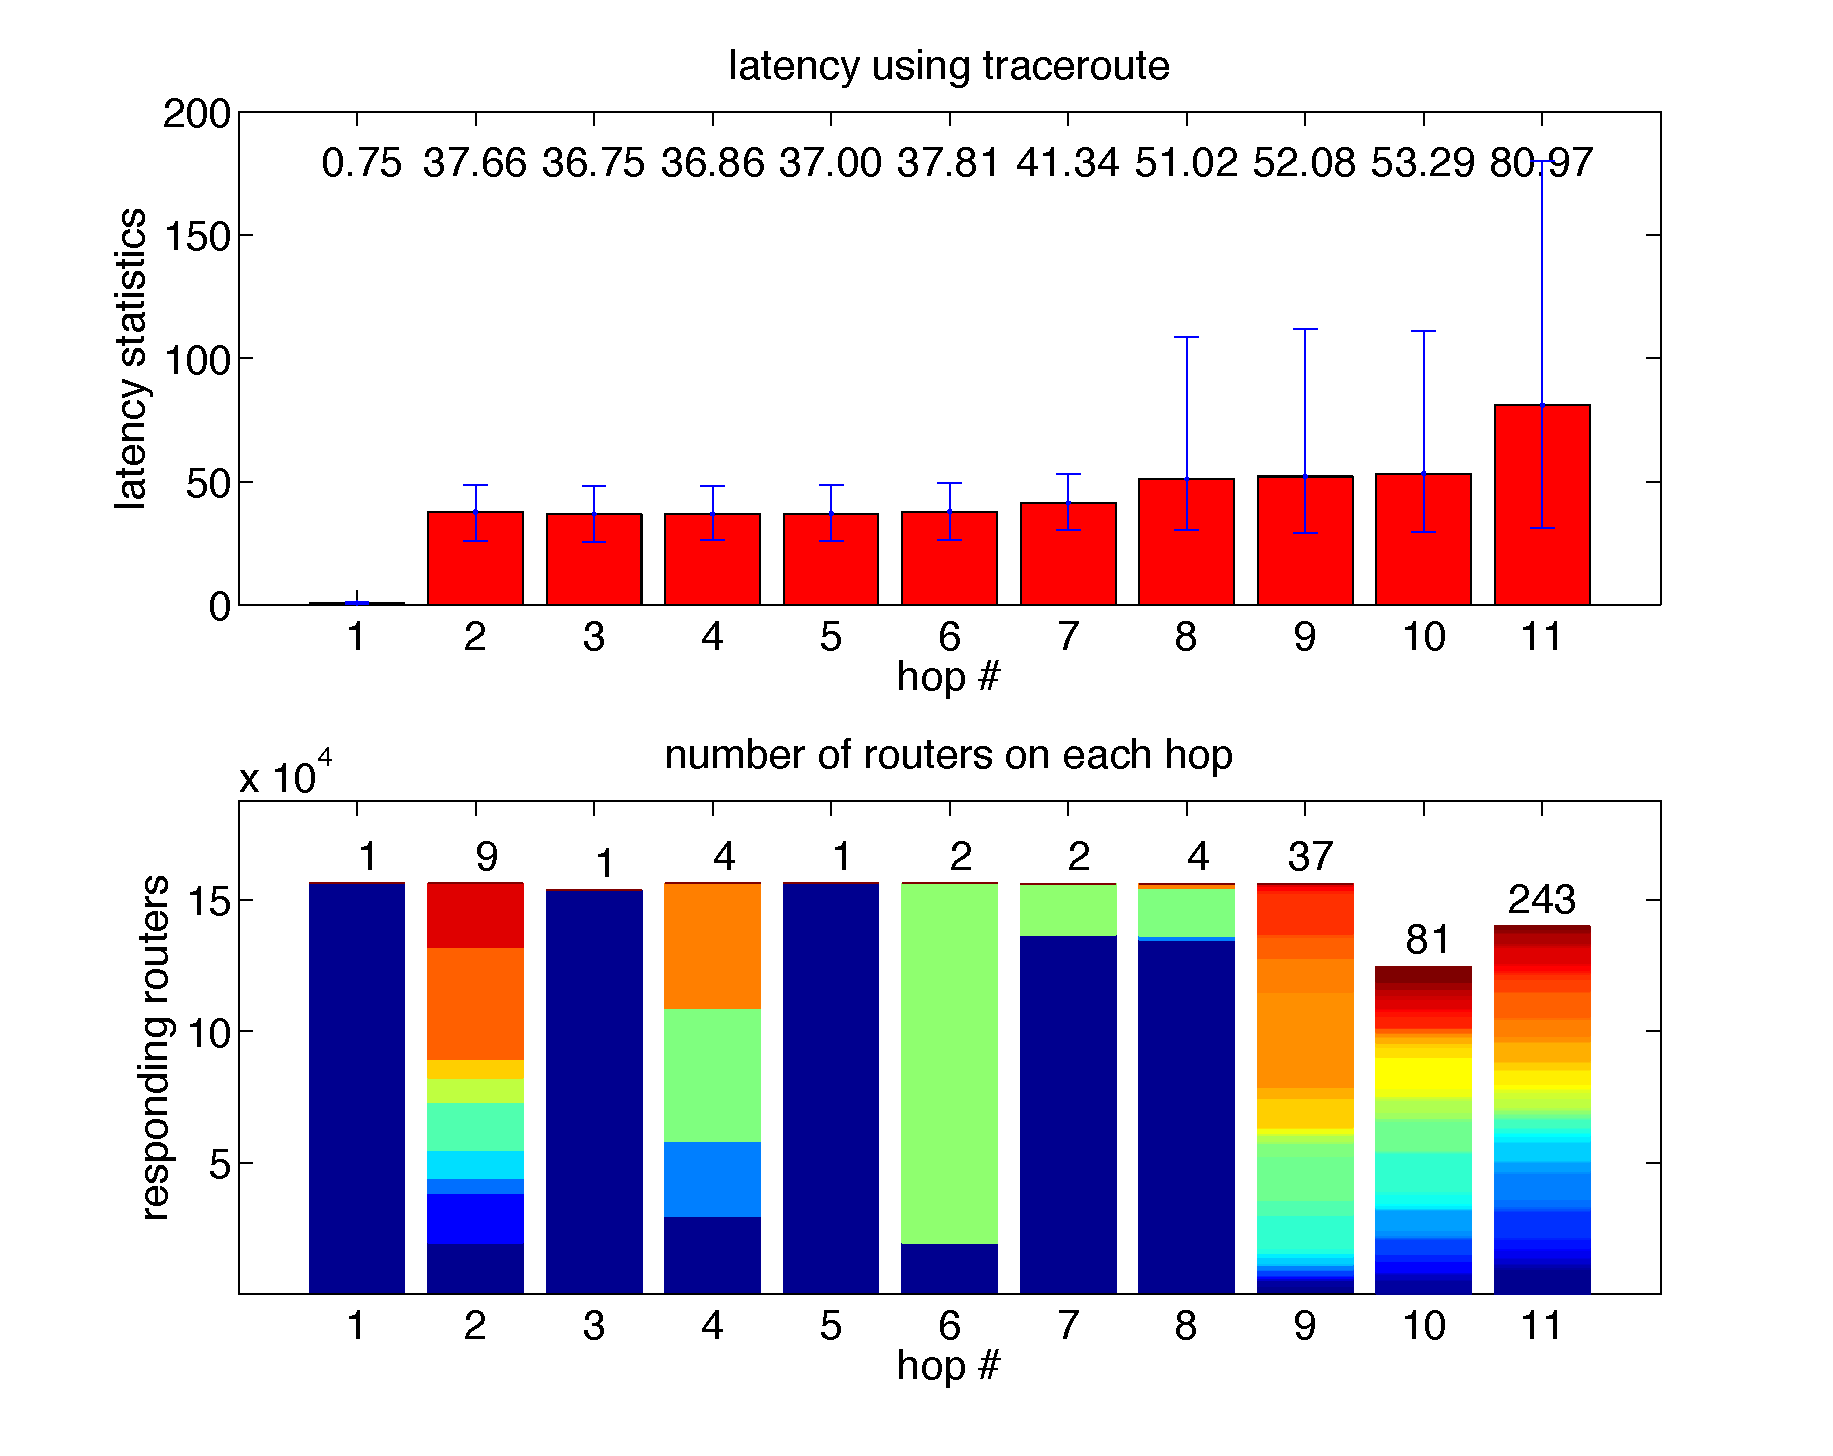
\includegraphics[width=\linewidth]{../figs/mobile_latency.pdf}
  \vspace{-1em}
  \caption{(Top) Latency measured in each hop of AT\&T cellular networks; (Bottom) The number of routers that responded on each hop}
  \label{fig:mobile_latency}
\end{figure}

We have found that within the cellular backbone and AT\&T's network (from the 2nd hop to 7th hops), the latencies are fairly stable at around 40 ms with variation of about 15 ms. There are also relatively few routers on a given hop. The second hop has 9 different responders, which are likely AGWs behind the eNode-B. They do not seem to change based on your location (as you can see in Fig\,\ref{fig:mobile_mobile} when we were moving between Berkeley and SF). We conjecture that the fourth hop might be comprised of four load balancers, as the fifth hop is consistent across all the measurements. After first 7 hops, the latency experiences a large increase, and the number of routers on each hop also increase dramatically.

\begin{figure}
  \centering
  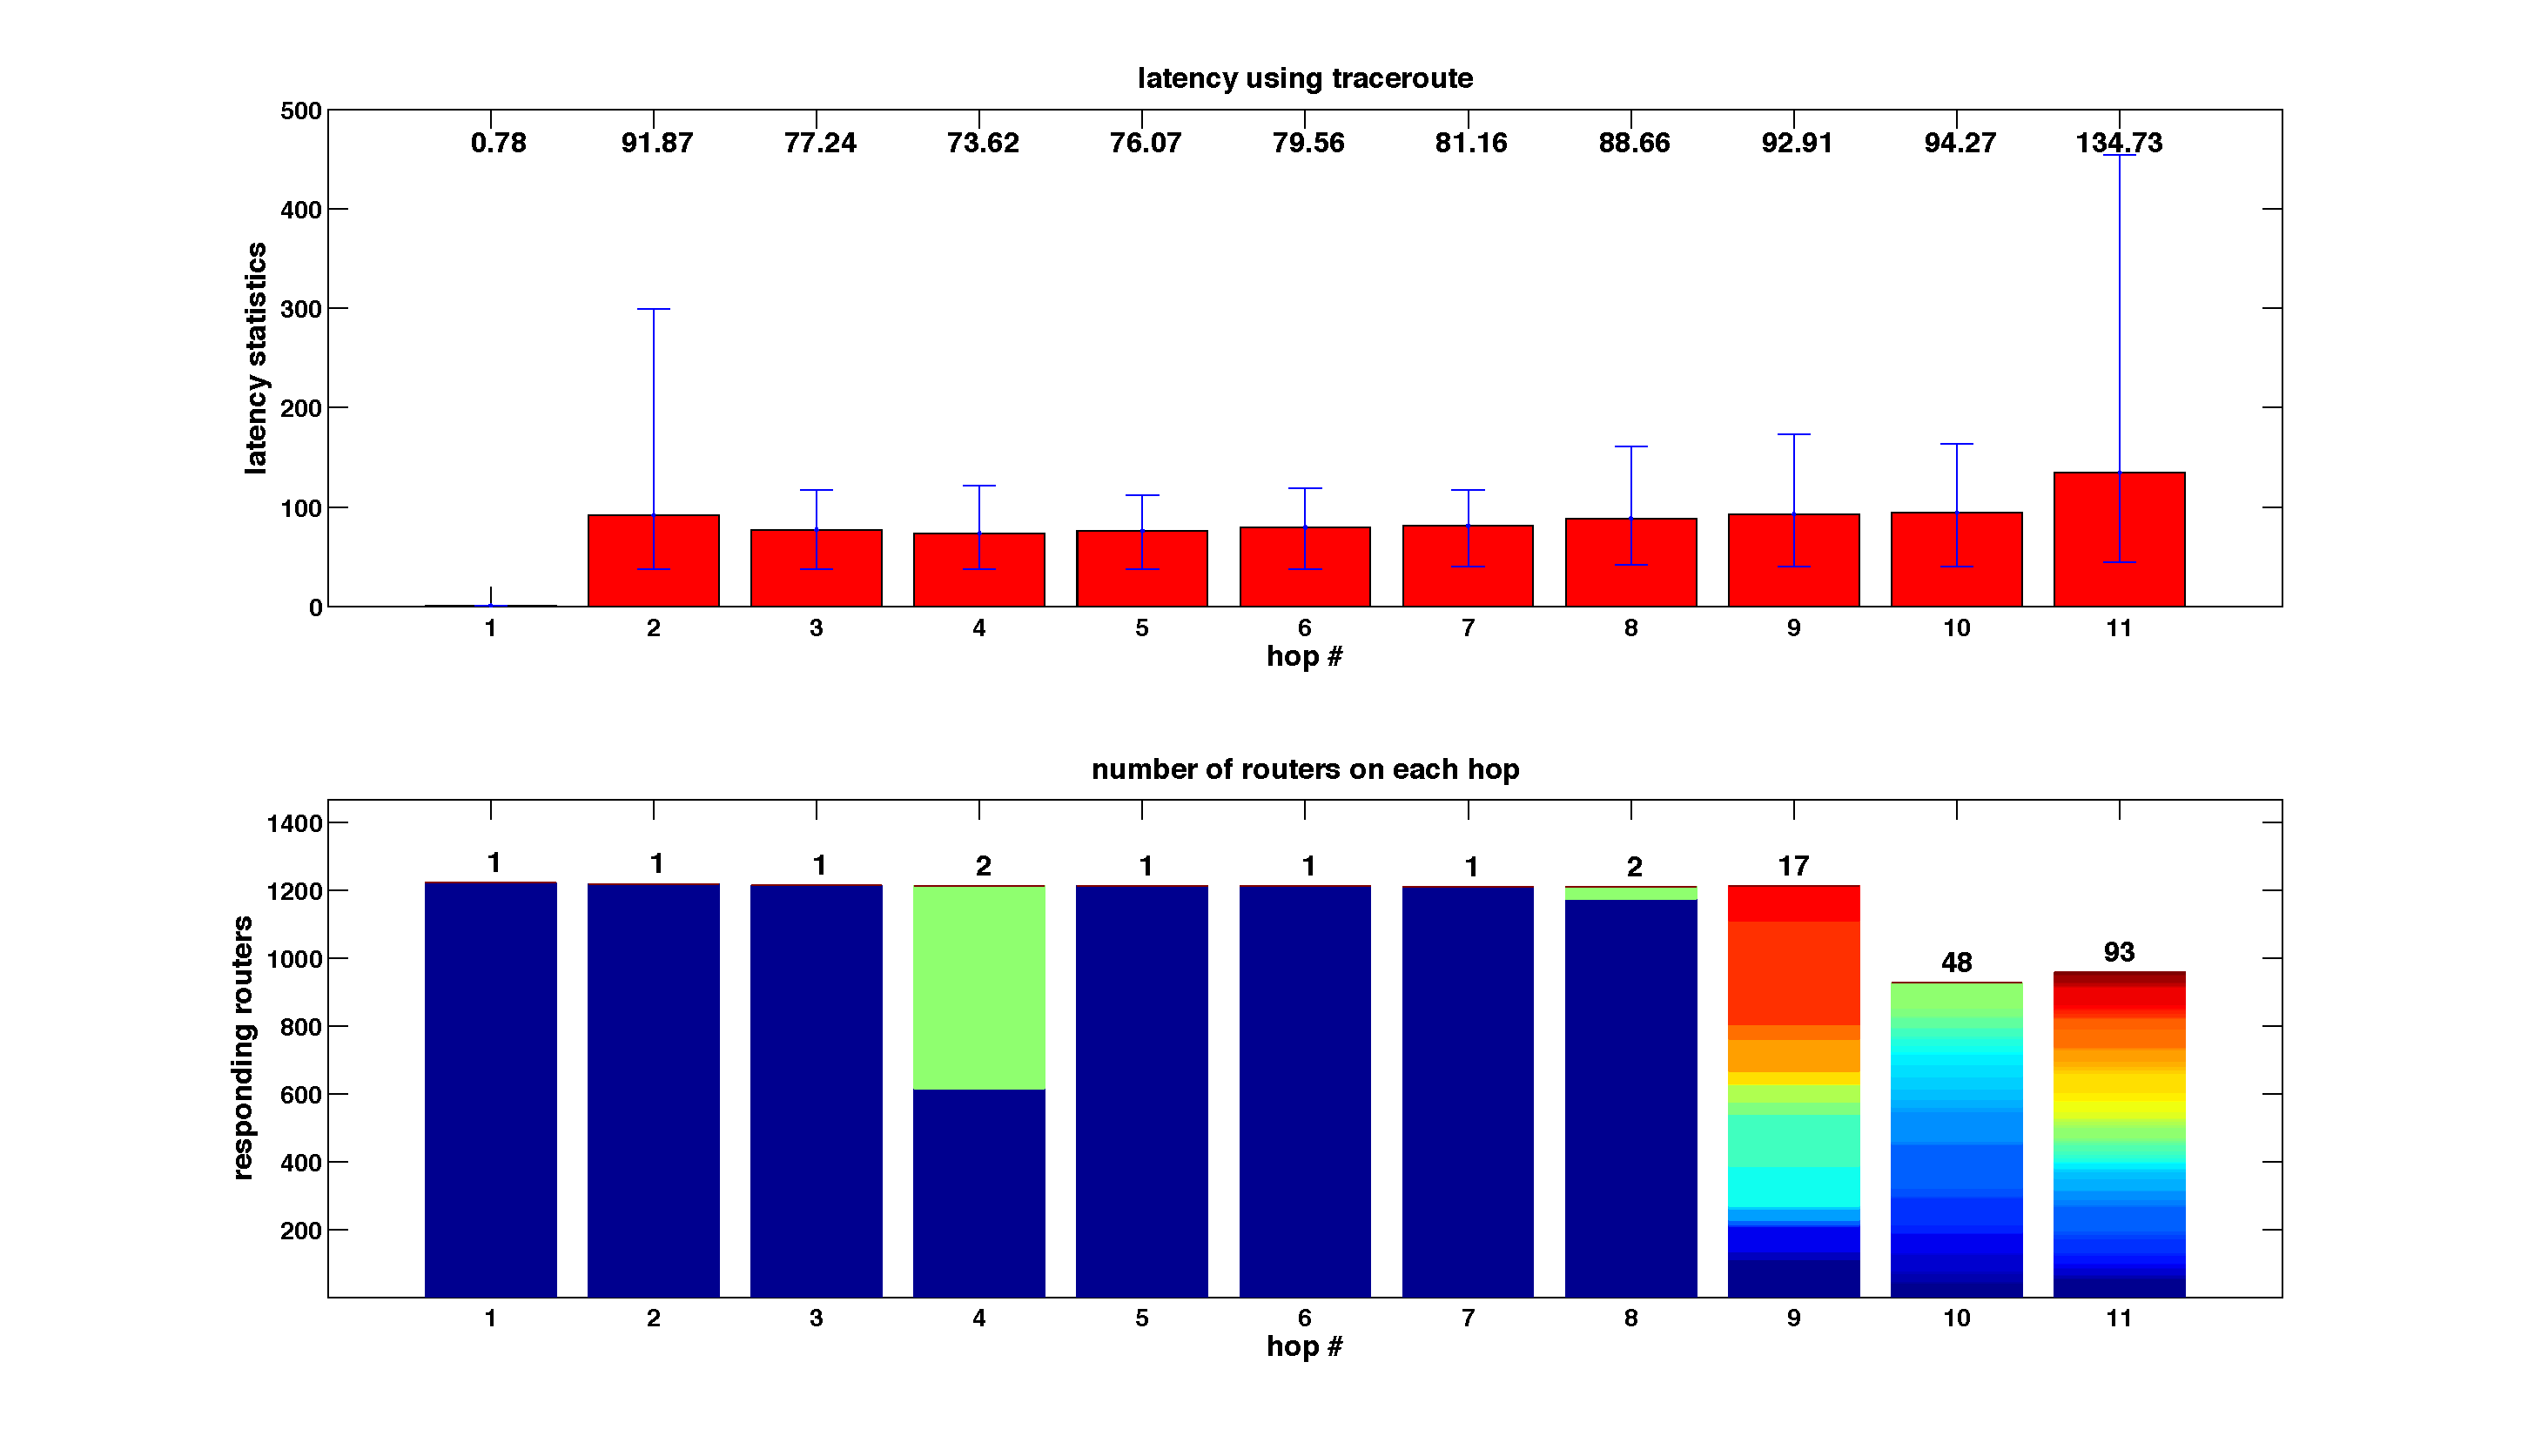
\includegraphics[width=\linewidth]{../figs/mobile_sfo.pdf}
  \vspace{-1em}
  \caption{Measurements conducted while moving between Berkeley and San Francisco.\\ (Top) latency measured in each hop of AT\&T cellular networks; (Bottom) the number of responding routers on each hop}
  \label{fig:mobile_mobile}
\end{figure}

From Fig.\,\ref{fig:mobile_mobile}, we find that the latencies are significantly larger when compared to Fig.\,\ref{fig:mobile_latency}. We believe that this is in part due to a difference in radio access technology -- during the majority of the journey, the mobile device utilized the 4G (HSDPA+) network rather than LTE. As can be seen, the latency on the second hop has increased significantly; we believe mobility accounts for part of the degradation. Once again the routing within the cellular backbone is fairly stable.

To further understand routing stability, we evaluate each trace. In a single {\textit traceroute} log, the routing might change; this rapidly-variable routing is called fluttering \cite{paxson1997measurements}. For each hop, we determine how many different routes the packet has taken, and draw this in a stacked bar plot (Fig.\,\ref{fig:mobile_fluttering}). The horizontal axis the hop number and the vertical axis counts the number of different routes in our measured data. For most of the routes within AT\&T's cellular backbone, the routes are fairly stable. When approaching the WAN (starting from hop 11), routing fluttering happens more frequently (likely due to the crossing of AS boundaries).

\begin{figure}
  \centering
  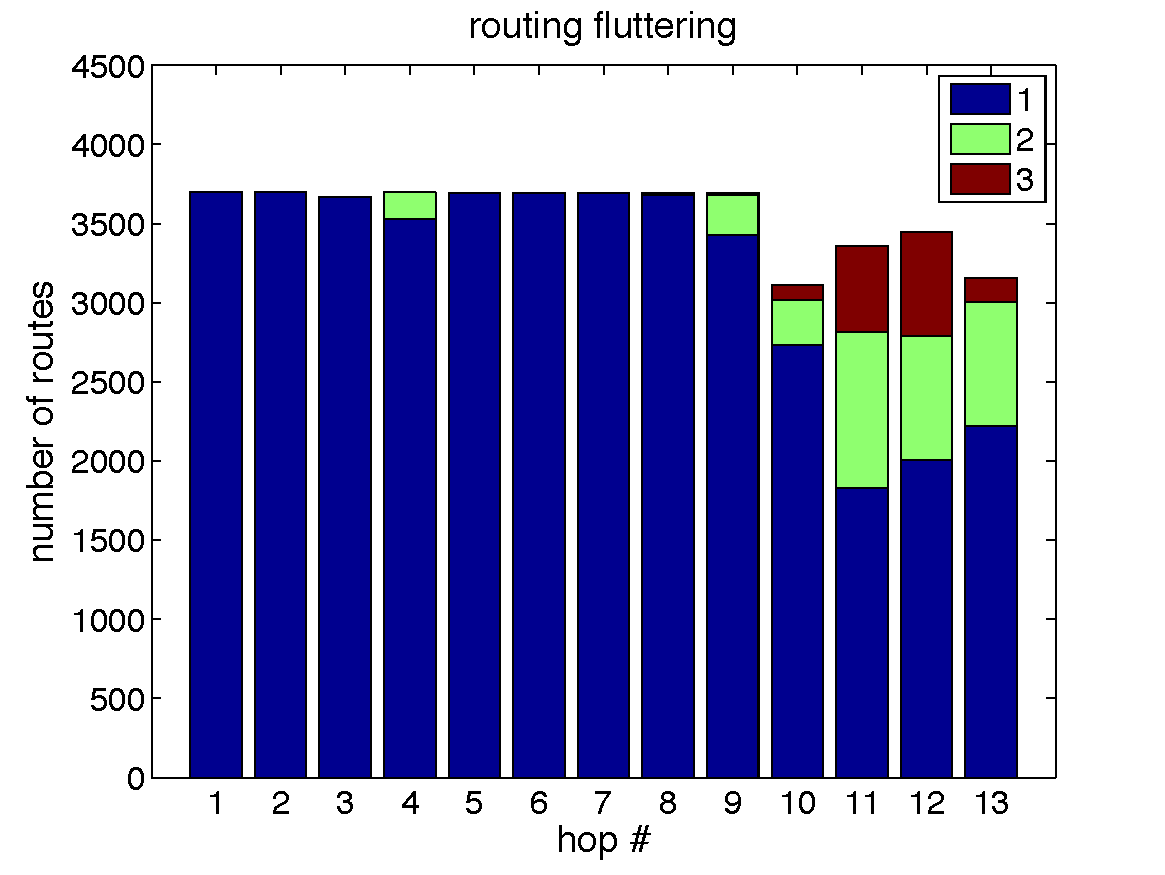
\includegraphics[width=\linewidth]{../figs/mobile_fluttering.pdf}
  \vspace{-1em}
  \caption{Routing fluttering within AT\&T cellular networks}
  \label{fig:mobile_fluttering}
\end{figure}

%%% Local Variables: 
%%% mode: latex
%%% TeX-master: "main"
%%% End: 
